\clearpage
\subsection{State observer}

In the simple example for a state space controller in figure \ref{fig:simpleProcess_Controller}, it was implied, that all state space variables can be measured. And these measured variables can be fed back in order to let the state space controller work. What if either a state variable can not be measured or the sensor costs too much to be economic?

David Gilbert Luenberger, working as professor at the Stanford University, invented a state observer called Luenberger observer. With this technique it is possible to use a state space controller, although not all state variable can be measured. 

\begin{figure}
	\centering
		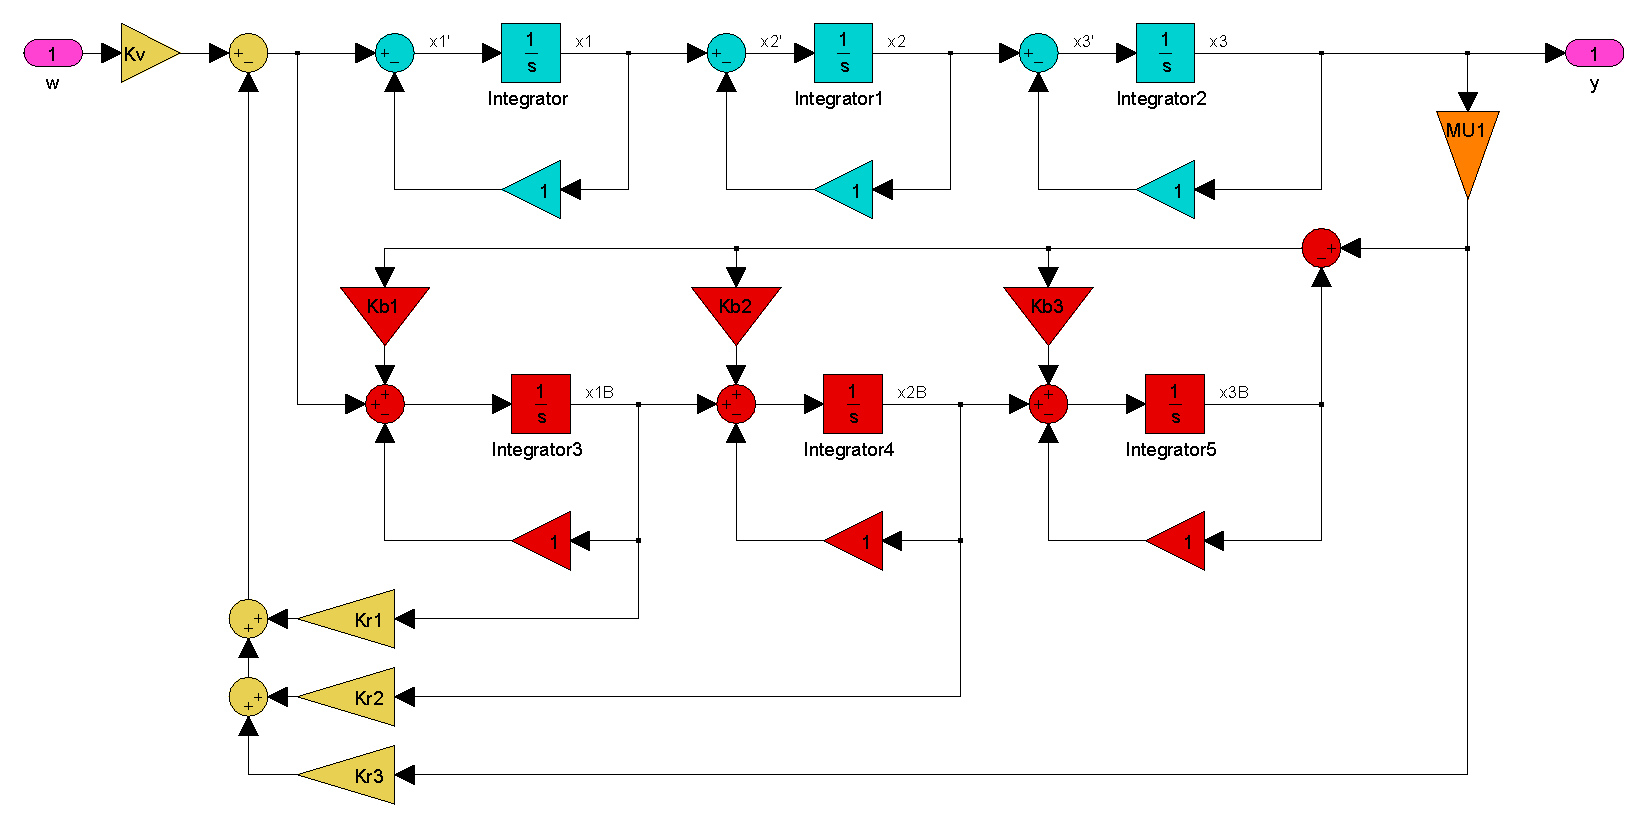
\includegraphics[width=1.00\textwidth]{03_Grafiken/simpleProcess_Controller_Observer.pdf}
	\caption{Simple process including a state space controller and an state observer}
	\label{fig:simpleProcess_Controller_Observer}
\end{figure}

In figure \ref{fig:simpleProcess_Controller_Observer} the state space controller is extended with an Luenberger observer. The observer is marked in red color. So, what exactly is shown there? To control the process with the standard state space controller, three measurement converters MUx are needed (\ref{fig:simpleProcess_Controller}). With the Luenberger observer, only one of them is required. In the example, there is a sensor for the output state variable. This state variable is fed back, just as common from the state space controller. But the other two state variables can not be measured, so the observer simulates the whole open loop process and implements this process in the controller. So the state variables \textit{x1B} and \textit{x2B} are fed back and if the observer poles are fast enough, the state space controller itself will not notice, that these state variables are not the original ones. These values are only estimated values but very good ones. To correct and stabilize the values of the observer, the measured value \textit{x3} is injected in the process and moves the simulated process in the right direction. This correcting works with the observer feedback factors \textit{Kbx}. 

Based on the fact, that the state space controller for the quadrocopter will not require an observer, this chapter will not be enlarged. 